\documentclass[final,t]{beamer}
\usepackage[scale=1.24]{beamerposter}
\usepackage{graphicx}
\usepackage{booktabs}
\usepackage{amsmath,amssymb}
\usepackage{geometry}

\geometry{
  paperwidth=48in,
  paperheight=36in,
  margin=1in
}

% Define colors
\definecolor{ColumbiaBlue}{RGB}{29, 79, 145}
\setbeamercolor{structure}{fg=ColumbiaBlue}
\setbeamercolor{headline}{bg=ColumbiaBlue,fg=white}
\setbeamercolor{block title}{bg=ColumbiaBlue,fg=white}
\setbeamercolor{block body}{bg=white,fg=black}

\graphicspath{{images/}}

% --- HEADER ---
\setbeamertemplate{headline}{
  \leavevmode
  \begin{beamercolorbox}[wd=\paperwidth]{headline}
    \begin{columns}[T]
      \begin{column}{.02\paperwidth}\end{column}
      \begin{column}{.15\paperwidth}
        \centering
        \vspace{1cm}
        
\includegraphics[height=4cm]{columbia_logo.png} 
        \vspace{1cm}
      \end{column}
      \begin{column}{.66\paperwidth}
        \centering
        \vspace{1cm}
        {\Huge \textbf{Semi-Supervised Latent Variable Model \\ for NYC Property Valuation}}\\[1.5ex]
        
        \begin{columns}[T]
          \begin{column}{0.45\textwidth}
            \centering
            {\Large \textbf{Daniel Lewis}}\\[0.5ex]
            {\large dl3645@columbia.edu}
          \end{column}
          \begin{column}{0.54\textwidth}
            \centering
            {\large STCS 6701: Probabilistic Models and Machine Learning}\\[0.5ex]
            {\large Professor Blei, Fall 2025}
          \end{column}
        \end{columns}
        
        \vspace{1cm}
      \end{column}
      \begin{column}{.15\paperwidth}
        \centering
        \vspace{1.5cm}
        
\includegraphics[height=3cm]{columbia_engineering_logo.png}
        \vspace{1.5cm}
      \end{column}
      \begin{column}{.02\paperwidth}\end{column}
    \end{columns}
  \end{beamercolorbox}
}

\begin{document}
\begin{frame}{}
  \vspace{-1.5cm}
  
  \begin{columns}[t]
    % --- COLUMN 1 ---
    \begin{column}{0.31\paperwidth}
      \begin{block}{Motivation \& Problem}
        Property valuation underpins \textbf{tax administration} to ensure fair revenue and \textbf{urban planning} to optimize resource allocation. We target both: taxation requires precise financial estimates, while planning uses value gradients to identify development zones.
        
        \textbf{Challenges}:
        \begin{itemize}
          \item \textbf{Heavy-tailed Distribution}: Prices exhibit extreme kurtosis of roughly 9.27, violating standard Gaussian assumptions.
          \item \textbf{Missingness}: About 25\% of records lack price data.
        \end{itemize}

        \textbf{Goal}: Learn a latent representation to predict sale prices and provide uncertainty estimates without discarding incomplete data.
      \end{block}

      \begin{block}{Methodology}
        We implement a \textbf{Semi-Supervised MIWAE} (SemiSupMIWAE) using a Student-$t$ Mixture Prior.

        \textbf{1. Generative Model}
        \begin{itemize}
          \item \textbf{Latent Space}: $z_i \sim \sum_{k=1}^K \pi_k \, t_\nu(\mu_k, \Sigma_k)$.
          \item \textbf{Covariates}: $x_i \mid z_i \sim \mathcal{N}\big(\mu_x(z_i), \operatorname{diag}(\sigma^2_x(z_i))\big)$.
          \item \textbf{Price Head}: $y_i \mid z_i \sim \mathcal{N}\big(\mu_y(z_i), \sigma^2_y(z_i)\big)$.
        \end{itemize}

        \textbf{2. Inference}
        We maximize the importance-weighted lower bound, the ELBO:
        \[
        \mathcal{L} \approx \mathbb{E}_{q_\phi} \left[ \log \frac{1}{K_{\text{IW}}} \sum_{k=1}^{K_{\text{IW}}} \frac{p_\theta(x_i, y_i \mid z_i^{(k)}) \, p(z_i^{(k)})}{q_\phi(z_i^{(k)} \mid x_i, y_i)} \right]
        \]
      \end{block}

      \begin{block}{Graphical Model}
        \begin{figure}
          \centering
          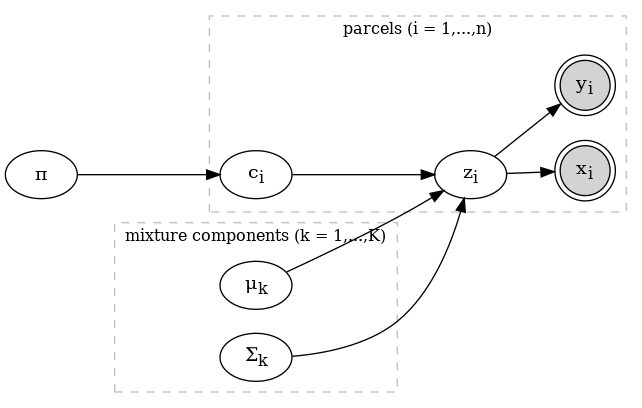
\includegraphics[width=0.95\textwidth]{miwae_graphical_model.png}
          \caption{SemiSupMIWAE Structure where $y$ is semi-observed.}
        \end{figure}
      \end{block}
    \end{column}
    
    % Spacer
    \begin{column}{0.02\paperwidth}\end{column}

    % --- COLUMN 2 ---
    \begin{column}{0.31\paperwidth}
      \begin{block}{Convergence \& Training}
        Trained on approximately 122,000 NYC parcels. Loss stabilizes around 50 epochs.
        \begin{figure}
          \centering
          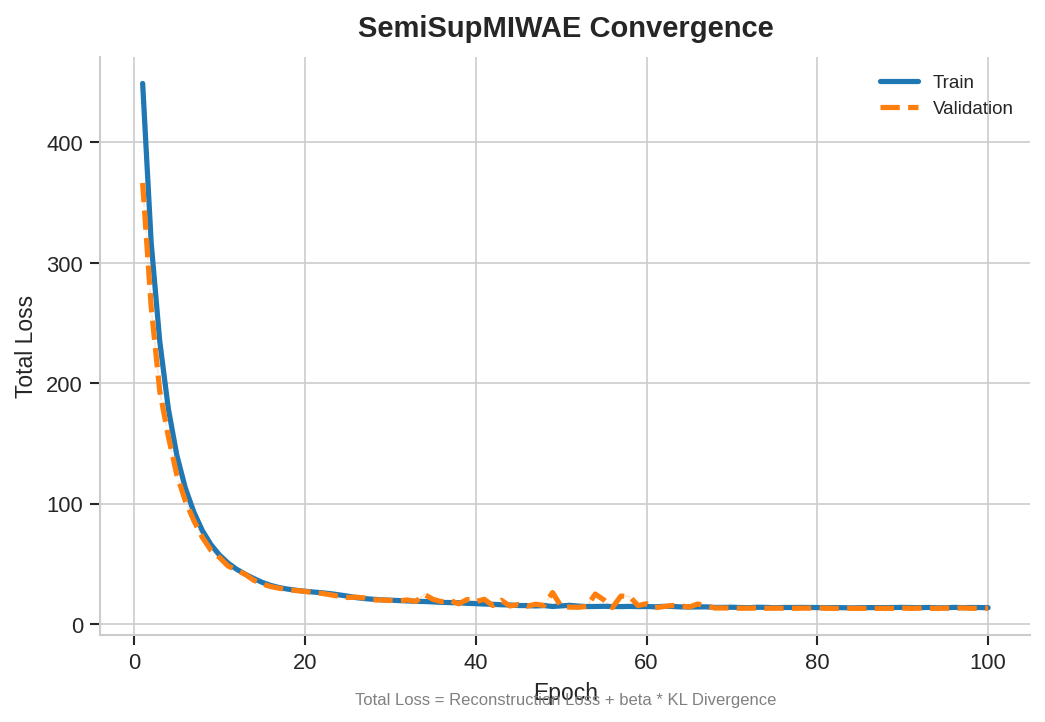
\includegraphics[width=0.9\textwidth]{convergence_loss.png}
          \caption{Training and Validation Loss on a Representative Fold.}
        \end{figure}
      \end{block}

      \begin{block}{Predictive Performance}
        Evaluated on a 20\% held-out set.
        
        \begin{table}
          \centering
          \begin{tabular}{lr}
            \toprule
            \textbf{Metric} & \textbf{Value} \\
            \midrule
            Avg. Log Posterior $p(y \mid x)$ & $-1.15$ \\
            RMSE & $\$24.6$ Million \\
            MAE & $\$2.18$ Million \\
            Median Absolute Error & $\$128,000$ \\
            \bottomrule
          \end{tabular}
          \caption{Predictive metrics.}
        \end{table}
      \end{block}

      \begin{block}{Residual Analysis}
        Residuals show significant heavy tails with Kurtosis approximately 9.27.
        \begin{figure}
          \centering
          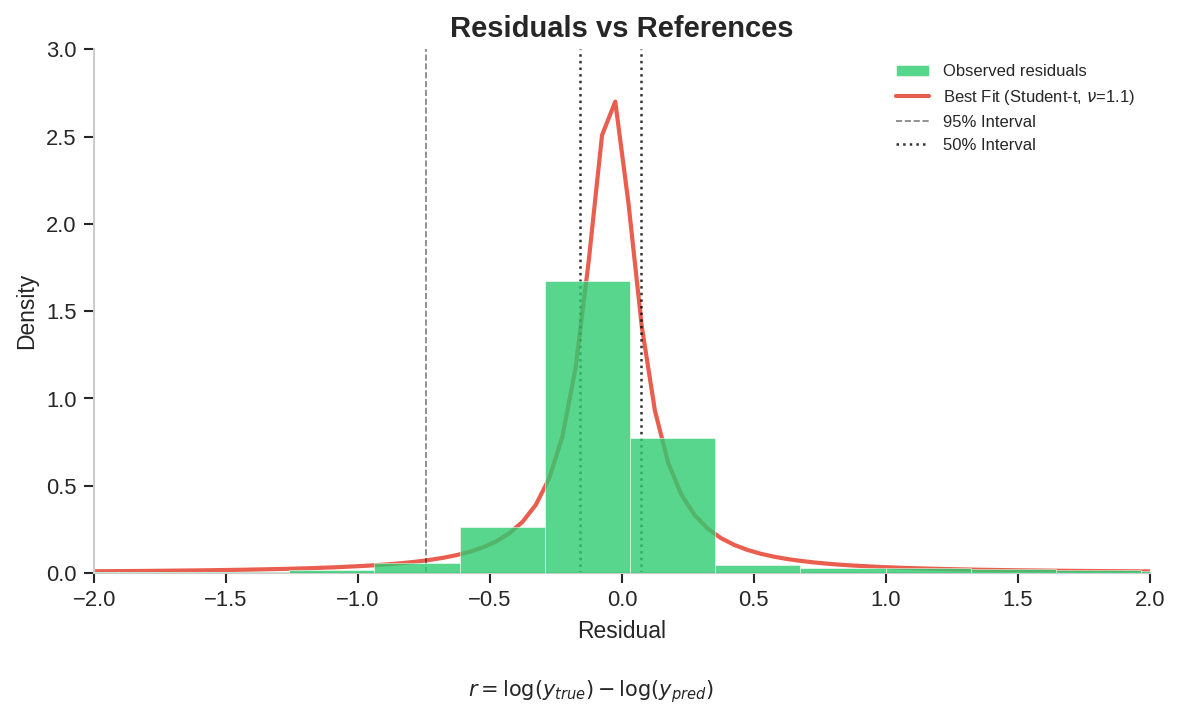
\includegraphics[width=0.48\textwidth]{residuals_hist_references.png}
          \hfill
          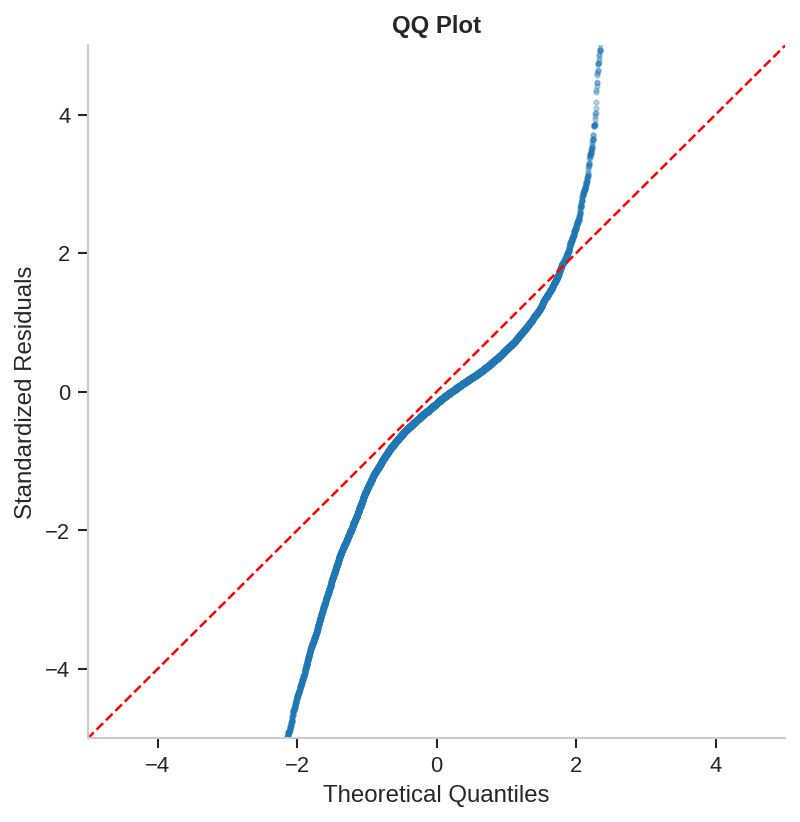
\includegraphics[width=0.48\textwidth]{residuals_qq.png}
          \caption{Log-price residuals vs Normal. Visual comparison highlights extreme kurtosis.}
        \end{figure}
      \end{block}
    \end{column}

    % Spacer
    \begin{column}{0.02\paperwidth}\end{column}

    % --- COLUMN 3 ---
    \begin{column}{0.31\paperwidth}
      \begin{block}{Latent Space Analysis}
        The 3D latent space, with $K=3$, captures interpretable structure.

        \textbf{1. Value Continuum}
        Gradient $z_0/z_1$ suggests a "Value/Size" factor.
        \begin{figure}
          \centering
          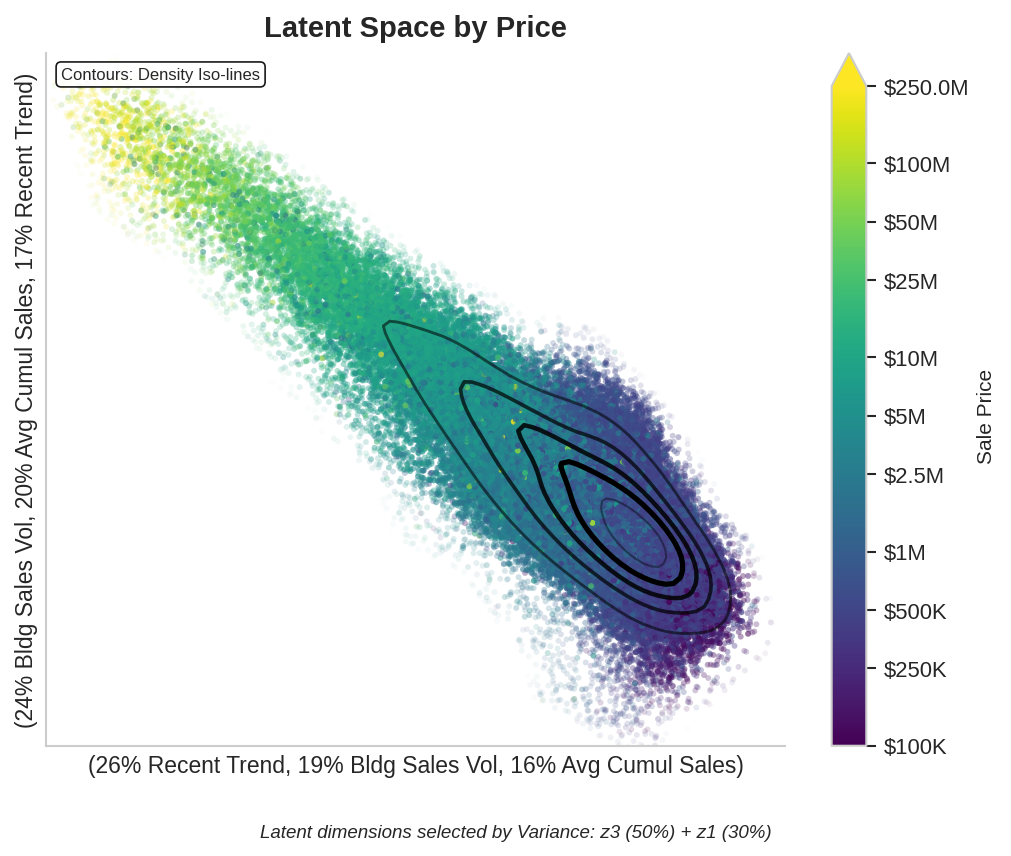
\includegraphics[width=0.9\textwidth]{latent_space_price.png}
          \caption{Latents colored by Price Decile.}
        \end{figure}

        \textbf{2. Structural Clustering}
        Clusters separate building classes such as Small vs Mixed-Use.
        \begin{figure}
          \centering
          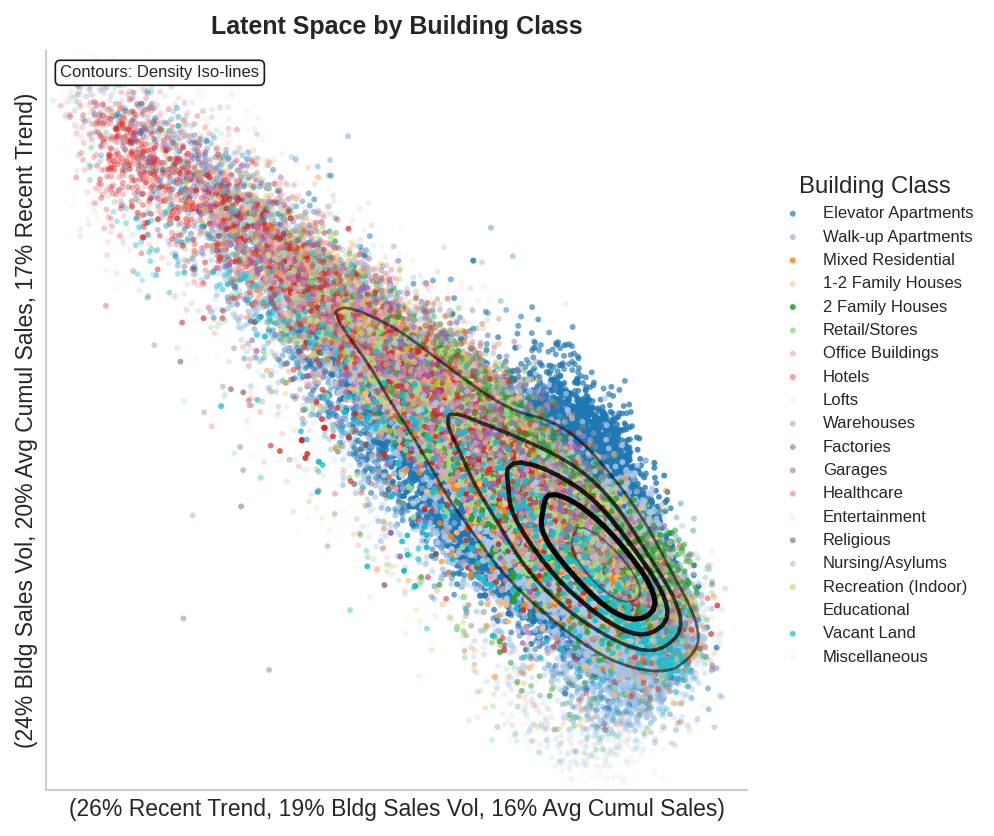
\includegraphics[width=0.9\textwidth]{latent_space_bldg.png}
          \caption{Latents colored by Building Class.}
        \end{figure}
      \end{block}

      \begin{block}{Discussion \& Future Work}
        \begin{itemize}
          \item \textbf{Findings}: Latents organize properties by value type, but Gaussian head misses tails with $R^2 \approx 0.27$ on residuals.
          \item \textbf{Future Work}:
            \begin{itemize}
              \item \textbf{Heavier Tails}: Replace Gaussian likelihood with Student-t.
              \item \textbf{Spatial}: Add Graph Neural Networks for neighborhood effects.
              \item \textbf{Visuals}: Overlay Gaussian on residual plots for kurtosis reference.
            \end{itemize}
        \end{itemize}
      \end{block}
    \end{column}
  \end{columns}
\end{frame}
\end{document}
